\documentclass{beamer}
%\documentclass[handout]{beamer} %handout para imprimir

\usetheme{JuanLesPins}
\usecolortheme{seahorse}
\usenavigationsymbolstemplate{}
%
\usepackage{color}
\usepackage{listings}
\usepackage[spanish]{babel}
\usepackage[utf8]{inputenc}
\usepackage{graphicx}
\usepackage{hyperref}
\usepackage{siunitx}
\usepackage[version=3]{mhchem}
\usepackage{multicol}

\title{Estudio de los Mecanismos Básicos de Electroporación a Través de la Modelación Numérica}
      
\author{Mauricio Alfonso}
\institute{DC - FCEyN - UBA}
%\date[12.2013]{SegInf, 2c - 2013}

%TODO cambiar la fecha

\begin{document}

\newcommand{\h}{\ce{H^+}}
\newcommand{\oh}{\ce{OH^-}}
\newcommand{\na}{\ce{Na^+}}
\newcommand{\cl}{\ce{Cl^-}}
\newcommand{\ontime}{\texttt{ON TIME}}
\newcommand{\offtime}{\texttt{OFF TIME}}
	
\frame {
	\titlepage
}

%TODO que aparezcan los items de a uno!!
%TODO carátula palabra numérica suelta
%TODO decidir si poner subsections o solo títulos (por ahora poner las dos cosas aunque quede feo)

\section{Introducción} 

\subsection{Introducción} 

\frame {
	%acá habría que poner algo basado en la introducción
	\begin{itemize}
		\item La \textbf{Electroporación} o \textbf{Electropermeabilización (EP)} es en la aplicación de pulsos eléctricos a una membrana biológica con el objetivo de incrementar su permeabilidad.
		\item De esta manera se facilita el ingreso de agentes terapéuticos a una célula.
		\item En la medicina se utiliza EP en la electroquimioterapia (ECT), la electrotransferencia génica (GET) y la electroporación irreversible (IRE).
		\item También tiene aplicaciones en el procesamiento de alimentos y la gestión ambiental. 
	\end{itemize}
}

\frame {
	% qué se hace y 4 partes
	En esta tesis se simula numéricamente la aplicación de pulsos eléctricos a una célula y se estudia su respuesta eléctrica, la permeabilización lograda y el transporte de especies iónicas. 
	
	\vspace{\baselineskip}

	Se estudiaron tres tipos de fenómenos físicos por separado:
	\begin{itemize}
		\item El potencial eléctrico en todo el dominio
		\item La creación y evolución de poros en la membrana celular
		\item El transporte de especies iónicas
	\end{itemize}
	
	Por último se analizaron todos los fenómenos acoplados.\\
}

\frame {
	% luego dominio y pulso
	\frametitle{Dominio}
	\begin{center}
		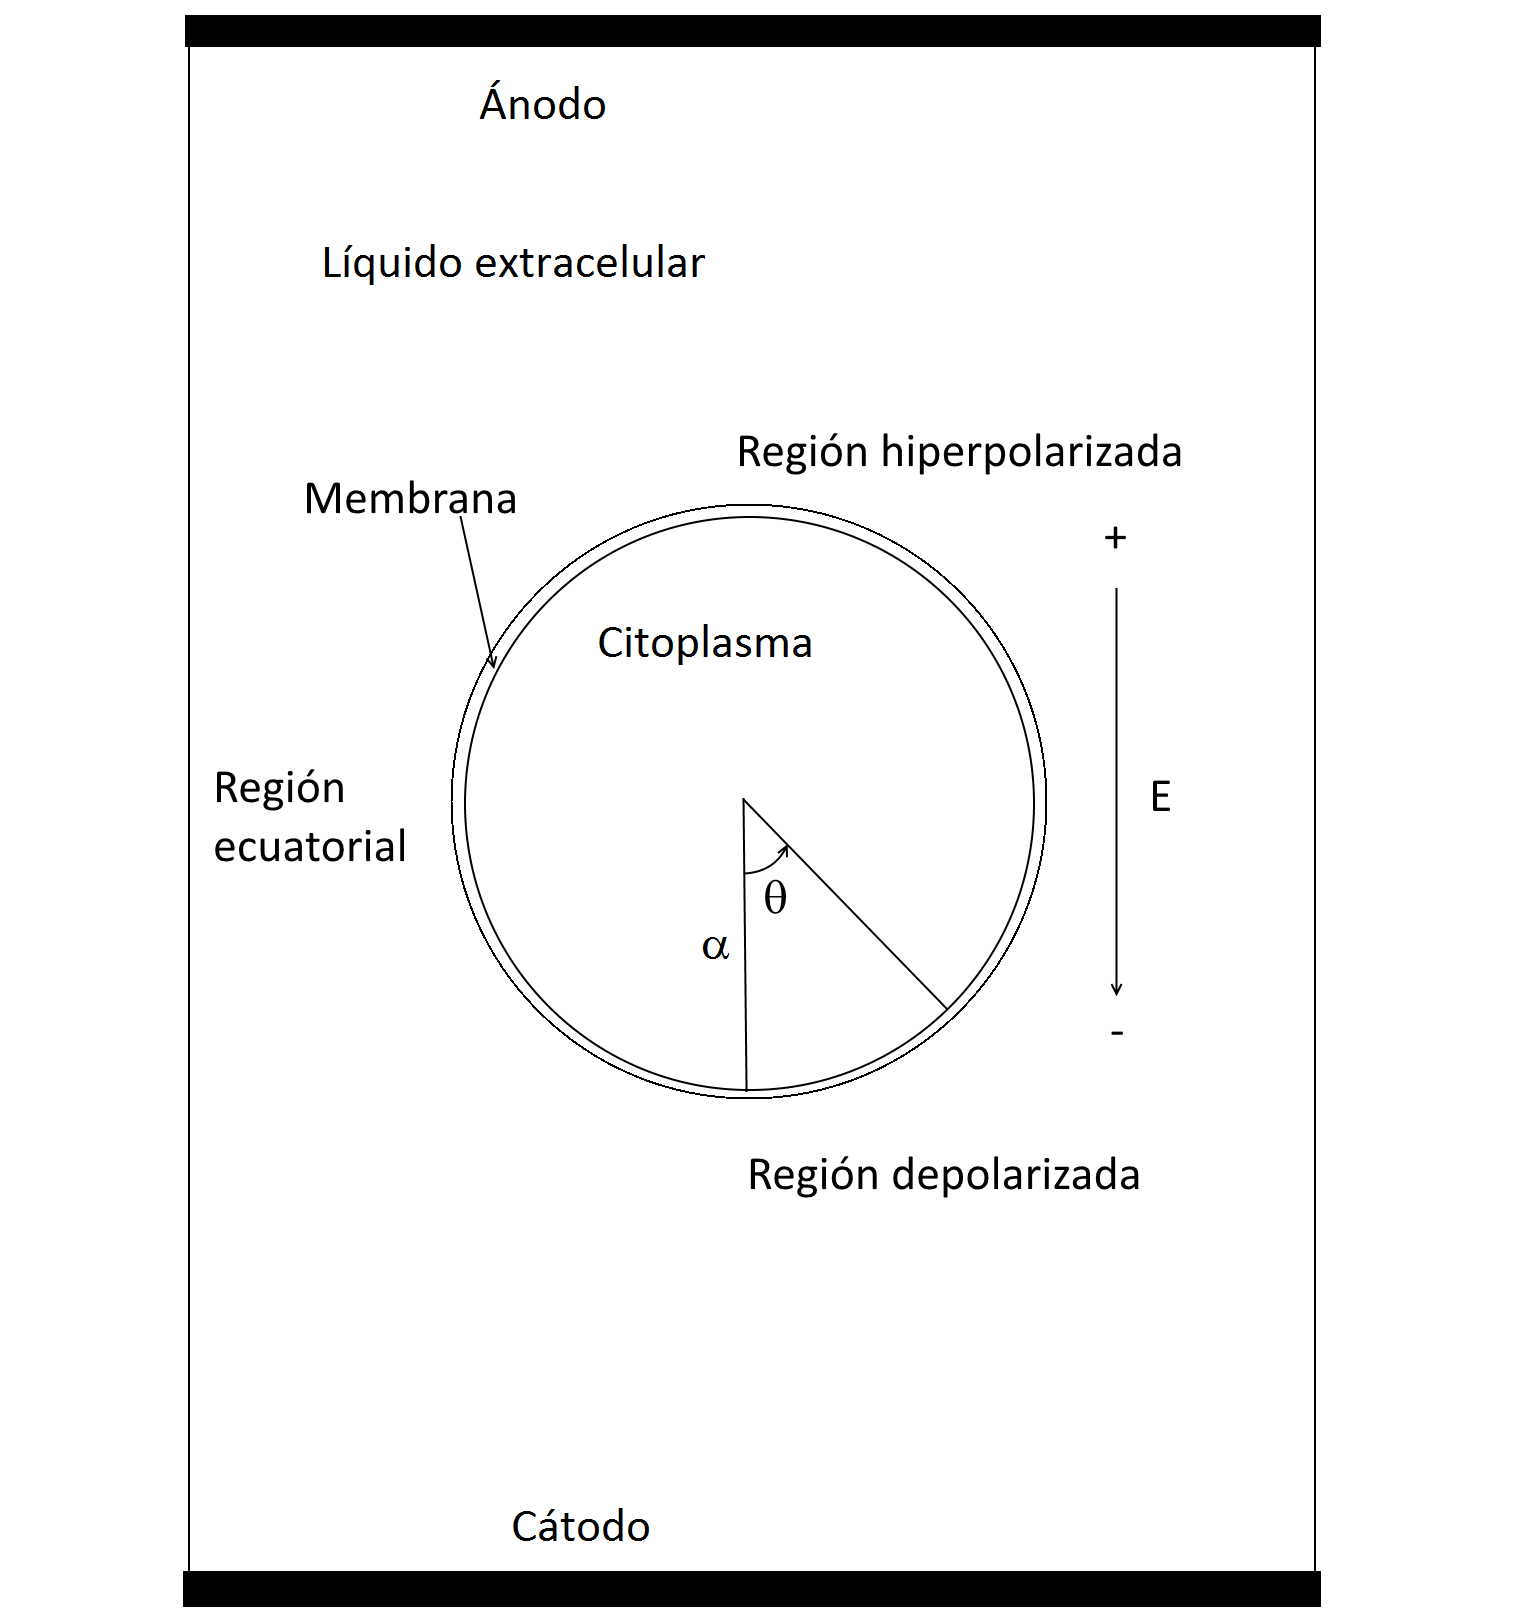
\includegraphics[keepaspectratio, height=0.88\textheight]{graficos/dominio}	
	\end{center}
}

\frame {
	\frametitle{Pulso Eléctrico}
	\begin{center}
		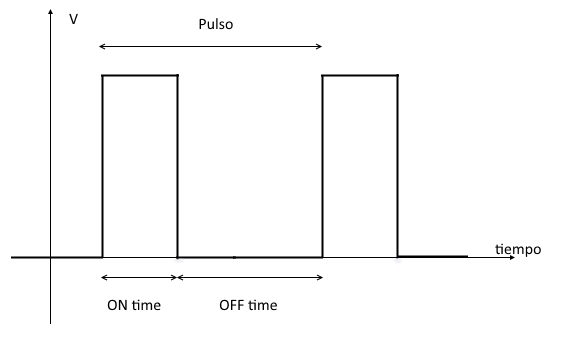
\includegraphics[keepaspectratio, width=0.75\textwidth]{graficos/pulso}	
	\end{center}
}


\frame {
	\frametitle{Detalles}
	\begin{itemize}
		\item Células esféricas de entre 10 y 50 \si{\micro\metre} de radio. \pause
		\item Membrana celular de 5 \si{\nano\metre} de espesor. \pause
		\item Pulsos eléctricos de hasta 2000 \si{\volt\per\centi\metre}, de 5 \si{\milli\second} de \ontime{} y 5 \si{\milli\second} de \offtime. \pause
		\item Se estudia la concentración de 4 especies iónicas: \h, \oh, \na{} y \cl.
	\end{itemize}
}

\section{Implementación}

%TODO corregir el C++ en negrita

\subsection{Métodos computacionales} \frame {
	%Mencionar FEM, Euler, C++, Eigen, OpenMP
	\frametitle{Métodos Computacionales}
	\begin{itemize}
		\item Se implementaron las simulaciones desde cero en \textbf{C++}.
		\pause
		\item Se utiliza principalmente el \textbf{Método de Elementos Finitos} y en menor medida diferencias finitas.
		\pause
		\item Se modela la membrana explícitamente, en lugar de considerarla una condición de borde.
		\pause
		\item Se trabaja en un dominio bidimensional con coordenadas cilíndricas.
		\pause
		\item Se hizo uso de la librería de álgebra lineal \textbf{Eigen} para \texttt{C++}.
		\pause
		\item Se paralelizaron partes del código en varios hilos con \textbf{OpenMP}.
		\pause
		\item Adicionalmente se utilizó \textbf{Python} y la librería \textbf{matplotlib} para procesar las salidas. 
	\end{itemize}
}

\subsection{Mallado} 

\frame {
	%Poner imágenes y explicar.
	\frametitle{Mallado}
	\begin{multicols}{2}
		\itemize{
			\item Coordenadas cilíndricas (2D)
			\item Elementos cuadrilaterales
			\item Tamaño variable de los elementos
			\item Generadas con AutoMesh2D
			\item Entre 7000 y 9000 elementos según la malla
			\vspace{1cm}
		}
		\columnbreak
		\begin{center}
			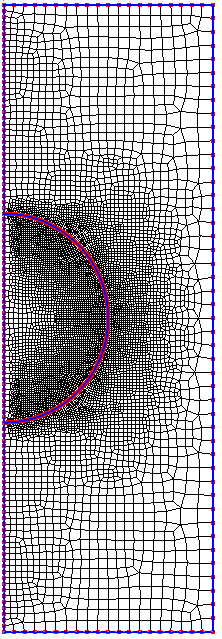
\includegraphics[keepaspectratio, height=0.85\textheight]{graficos/meshfar} \\
		\end{center}
	\end{multicols}
}

\frame {
	\frametitle{Mallado (detalle)}
	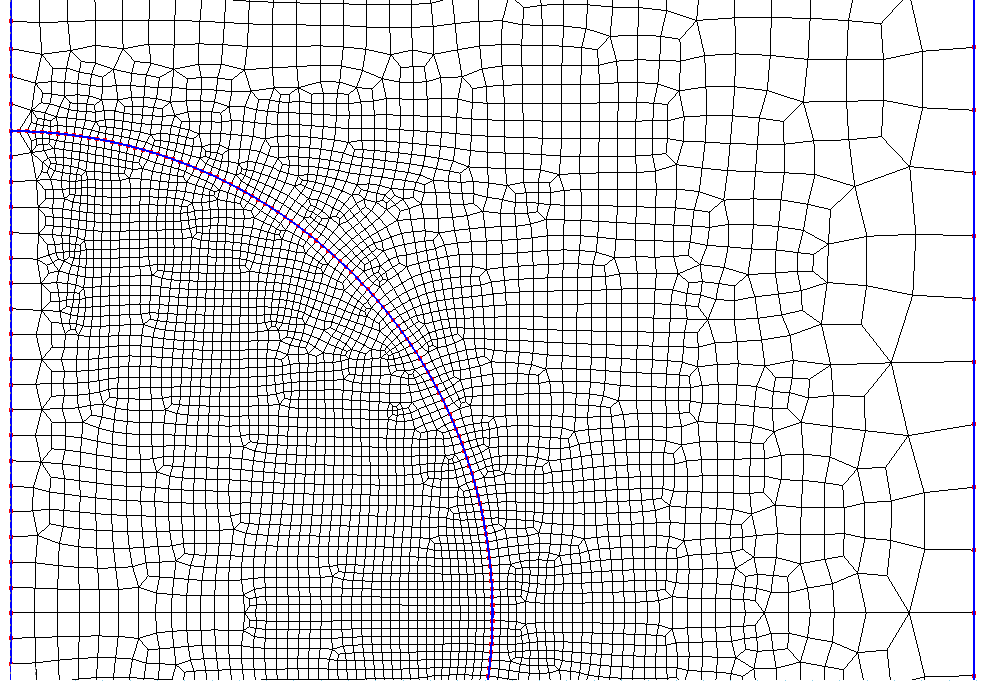
\includegraphics[width=\textwidth]{graficos/meshclose}
}

\frame {
	\frametitle{Mallado (membrana)}
	La membrana se modela explícitamente en la malla con dos elementos de ancho en la dirección radial. \\
	\vspace{0.25\baselineskip}
	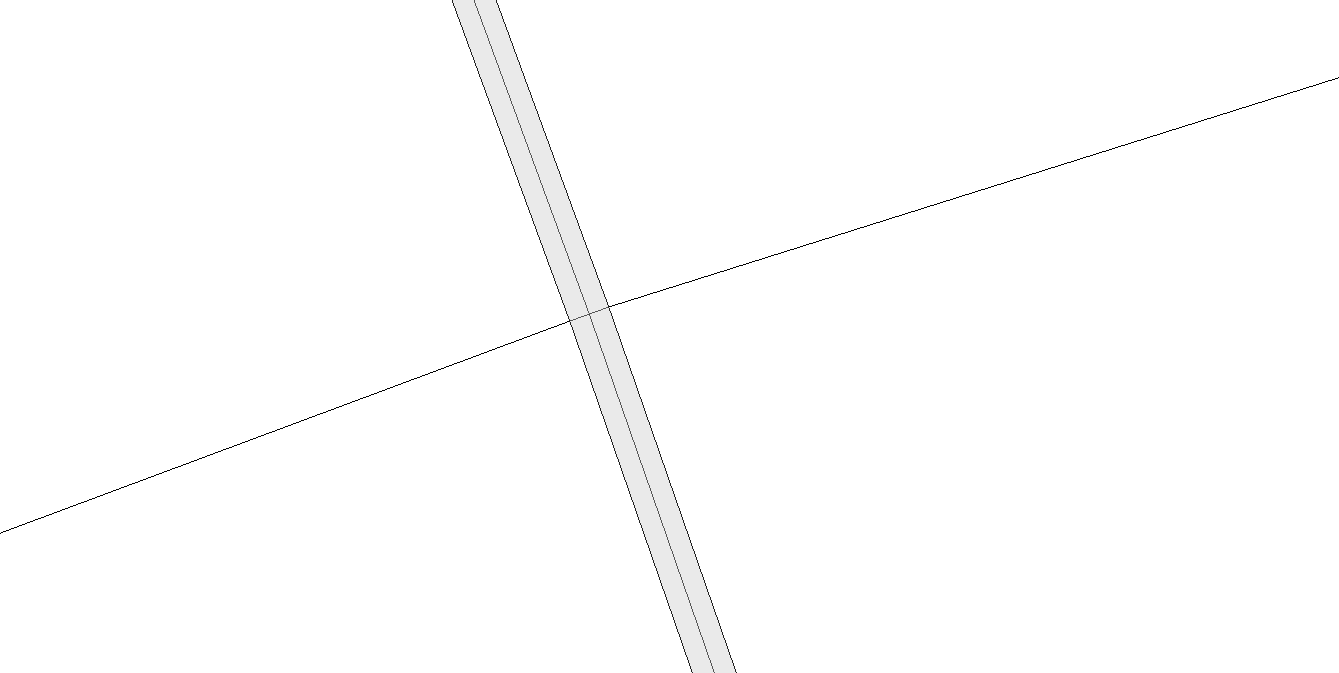
\includegraphics[width=\textwidth]{graficos/meshmembrane}
}

\section{Potencial Eléctrico}

\subsection{Teoría} \frame {
	%Fórmulas
	\frametitle{Potencial Eléctrico}
	Ecuación de Poisson:
	\begin{equation*}
		\nabla \sigma_{elem} \cdot (\nabla \phi) = 0 
	\end{equation*}
	El potencial transmembrana (PTM) puede aproximarse a:
	\begin{equation*}
		 V^{\theta} = f_s\, E\, \alpha\, \cos (\theta) 
	\end{equation*}
	Condiciones de borde de Dirichlet en los electrodos y de Neumann en el borde restante.
}

\subsection{Resultados} 

\frame {
	Potencial eléctrico en el dominio
}

\frame {
	Campo eléctrico
}

\frame {
	ITV
}

\section{Poros} 

\subsection{Teoría} \frame {
	Fórmulas
}

\subsection{Resultados}

\frame {
	histogramas. quizás hacer videos de los histogramas?
}

\frame {
	itv en función del ángulo y en función del tiempo. Estaría muy bueno poner videos para que se entienda.
}

\section{Transporte}

\subsection{Teoría} \frame {
	Fórmulas
}

\subsection{Resultados} \frame {
	Gráficos de resultados. Explicar que no sirven para nada.
}

\section{Acoplado}

\subsection{Teoría} \frame {
	Fórmulas. podría ir también un poco de implementación?
}

\subsection{Resultados un pulso} \frame {
	videos
}

\subsection{Resultados varios pulsos} 

\frame {
	videos muy grosos. También podrían ir videos de los histogramas.
}

\section{Escalabilidad}

\subsection{Escalabilidad} \frame {
	Mencionar como se usa openmp y resultados
}

\section{Conclusiones} 

\subsection{Conclusiones} \frame {
	Conclusiones
}

\subsection{Trabajo Futuro} \frame {
	Trabajo Futuro
}

\end{document}
